%% deferred_followup.tex — material PARKED for the follow-up paper.
%%
%% Per the project lead's decision of 2026-09-08, the Physics of Fluids
%% benchmark paper (main.tex) is scoped to THREE regimes: cylinder wake,
%% 2D Kolmogorov turbulence, and JHU 3D isotropic turbulence. The FireBench
%% (3D multiphysics wildfire LES, corrupted measurement operators) and
%% SHIFT-WING (unstructured wing geometry, surface-only sensing) regimes are
%% deferred to a follow-up paper. Every block below was cut VERBATIM from
%% main.tex on that date, preceded by a comment naming the section it came
%% from. Nothing here is \input from main.tex; it is a holding file only.
%% Bibliography keys used here (firebench2024, luminary2026shiftwing) remain
%% in references.bib / refs_extra.bib.


% ---- cut from tab:regimes (sec:datasets), rows for FireBench and SHIFT-WING, 2026-09-08 ----
% These two table rows sat between the JHTDB row and \end{tabular}.
3D multiphysics & FireBench\cite{firebench2024} & $3.7{\times}10^{6}$ & $u,v,w,\theta,\rho_f$ & temp.\ block & corrupted operators \\
3D geometry & SHIFT-WING\cite{luminary2026shiftwing} & $4{\times}10^{5}$/case & $U_x,U_y,U_z,C_p$ & by case & surface-only sensing \\

% ---- cut from sec:datasets, \paragraph{Wildfire LES.}, 2026-09-08 ----
\paragraph{Wildfire LES.} From the public FireBench store,\cite{firebench2024}
the two large-eddy simulations at 10 and 12\,m/s driving wind; we extract a
$152\times126\times192$ region around the fire front ($3.7\times10^{6}$
points; velocity, potential temperature $\theta$, fuel density $\rho_f$; 120
snapshots, temporally blocked split with a 10-frame guard gap). Sensors
observe the three wind components; the thermochemical channels are inferred.
This is the operator-realism regime: evaluation applies noise, slab occlusion,
and channel dropout to the sensor sets (Sec.~\ref{sec:sensors}).

% ---- cut from sec:datasets, \paragraph{Unstructured wing meshes.}, 2026-09-08 ----
\paragraph{Unstructured wing meshes.} SHIFT-WING:\cite{luminary2026shiftwing}
673 converged RANS cases over transport-aircraft wing--fuselage variants
spanning Mach 0.5--0.85, incidence 0.02--3.99$^\circ$, and 40 geometry
parameters. Each case carries $4\times10^{5}$ near-body volume nodes and a
$6.5\times10^{4}$-node surface pool with pressure and wall shear; observations
are surface-only (512 pressure taps $+$ 128 shear gauges drawn from the skin),
and the target is the volumetric field. Split 600/73 by case. This regime is
the capability filter: methods whose interface cannot accept an unstructured,
case-varying point cloud with surface-confined sensors cannot enter without
resampling artifacts, and their rows are reported as not applicable rather
than silently omitted.

% ---- cut from tab:capability (sec:methods), original five-column capability matrix, 2026-09-08 ----
% main.tex now carries a three-column (Cyl./Kolm./JHU) version of this table; the Fire and Wing columns are preserved here.
\begin{table}[tbp]
\caption{\label{tab:capability}Capability matrix: which method families can
honestly enter which regimes. RS = requires resampling to a grid (lossy near
boundaries/meshes); --- = interface cannot express the task.
\todo{finalize per-method rows once the 2D fleet lands; consider expanding to
one row per method.}}
\begin{ruledtabular}
\begin{tabular}{lccccc}
Family & Cyl. & Kolm. & JHU & Fire & Wing \\
\hline
Interpolation/POD anchors & \checkmark & \checkmark & \checkmark & \checkmark & \checkmark \\
Point-attention det.\ (Senseiver) & \checkmark & \checkmark & \checkmark & \checkmark & \checkmark \\
Grid det.\ (FNO-class) & RS & \checkmark & \checkmark & \checkmark & --- \\
DeepONet-class & \checkmark & \checkmark & \checkmark & \checkmark & \checkmark \\
Latent-grid generative (LFM) & RS & \checkmark & \checkmark & \checkmark & --- \\
Latent neural-field gen.\ (CoNFiLD) & \checkmark & \checkmark & \checkmark & \checkmark & \checkmark \\
Voxel/video diffusion (Gen4Turb, S3GM) & RS & \checkmark & \checkmark & \checkmark & --- \\
Point-token generative (SiT-point) & \checkmark & \checkmark & \checkmark & \checkmark & \checkmark \\
Ambient point-cloud FM (\dmfgen{}) & \checkmark & \checkmark & \checkmark & \checkmark & \checkmark \\
\end{tabular}
\end{ruledtabular}
\end{table}

% ---- cut from sec:jhu, closing clause of the headline paragraph, 2026-09-08 ----
% Original clause "corrupted operators (Sec.~\ref{sec:firebench})" was dropped from the list of ill-posed payoffs.
payoffs concentrate where the problem is ill-posed --- unobserved channels,
corrupted operators (Sec.~\ref{sec:firebench}), sparser sensing --- and in

% ---- cut from sec:firebench (entire subsection incl. tab:ops and fig:qual-fb), 2026-09-08 ----
\subsection{Multiphysics LES under corrupted operators}\label{sec:firebench}

% Ported from iclr2027 Table tab:ops + robust-vs-clean ablation
\begin{table*}[tbp]
\caption{\label{tab:ops}Wildfire LES ($3.7$M points, 5 fields) under
realistic measurement operators (relative $L_2$ of ensemble mean / fair CRPS;
$K{=}8$, 8 snapshots, identical seeded operator realizations for all
methods). Sensors observe the three wind components at ${\sim}$1\% of points;
$\theta$ and $\rho_f$ are never observed. \dmfgen{} is a single amortized
model across all rows. The noise-$0.3\sigma$ row is out of distribution for
it (training noise reached $0.1\sigma$). Baseline cells are the
frame-matched re-evaluation (identical absolute frames and seeded operator
realizations for all methods; a frame-index audit found the original
baseline evaluation used an earlier window of the same held-out tail and
mildly flattered the baselines --- see the released audit trail).}
\begin{ruledtabular}
\begin{tabular}{lcccccc}
& \multicolumn{2}{c}{\dmfgen{}} & \multicolumn{2}{c}{Latent FM} & \multicolumn{2}{c}{Senseiver} \\
Operator & Rel.\ $L_2$ & CRPS & Rel.\ $L_2$ & CRPS & Rel.\ $L_2$ & CRPS \\
\hline
Clean & \textbf{0.456} & \textbf{0.234} & 0.719 & 0.482 & 0.840 & 0.608 \\
Noise $\sigma{=}0.1$ & \textbf{0.458} & \textbf{0.237} & 0.718 & 0.482 & 0.840 & 0.609 \\
Noise $\sigma{=}0.3$ & \textbf{0.461} & \textbf{0.248} & 0.721 & 0.484 & 0.840 & 0.610 \\
Slab occlusion (25\%) & \textbf{0.511} & \textbf{0.275} & 0.731 & 0.491 & 0.840 & 0.609 \\
Channel dropout ($u$ only) & \textbf{0.603} & \textbf{0.355} & 0.776 & 0.474 & 0.923 & 0.671 \\
\end{tabular}
\end{ruledtabular}
\end{table*}

Table~\ref{tab:ops} isolates operator realism on a regular LES extraction
(grid methods participate on their native terms). The amortized point-cloud
model wins every cell, and the reading of the baselines' apparent stability
matters more than the win: their numbers barely move across rows because they
are bias-dominated --- a model that extracts little of the information in the
sensors loses little when that information is corrupted. The latent baseline
reconstructs at 0.72--0.78 relative $L_2$ across all operators (predicting
zero scores 1.0), and its CRPS \emph{improves} slightly under channel
dropout only because its spread is large where its mean is wrong. Graceful monotone degradation,
not invariance, is the behavior a practitioner should want from a
reconstruction system, and only the model that uses the sensor information
exhibits it. A clean-trained control separates the mechanisms: it matches the
operator-amortized model under noise and occlusion (robustness there is
architectural) but collapses under channel dropout (0.743 vs.\ 0.603), the
one operator that changes the structure of the observation set --- and
operator-amortized training costs nothing in the clean condition (0.455 vs.\
0.456). Cross-variable inference falls out of the same interface: from wind
alone, unobserved fuel density is recovered at 0.044 relative $L_2$
(fire-front localization) and potential temperature at 0.49, and the
predictive standard deviation concentrates on the burn front --- $7$--$25\times$
its ambient value over the hottest 5\% of the domain --- which the model
never observes (Fig.~\ref{fig:qual-fb}).
\todo{add one voxel-diffusion row (Gen4Turb-class) for route completeness per
the gap analysis.}

\begin{figure}[tbp]
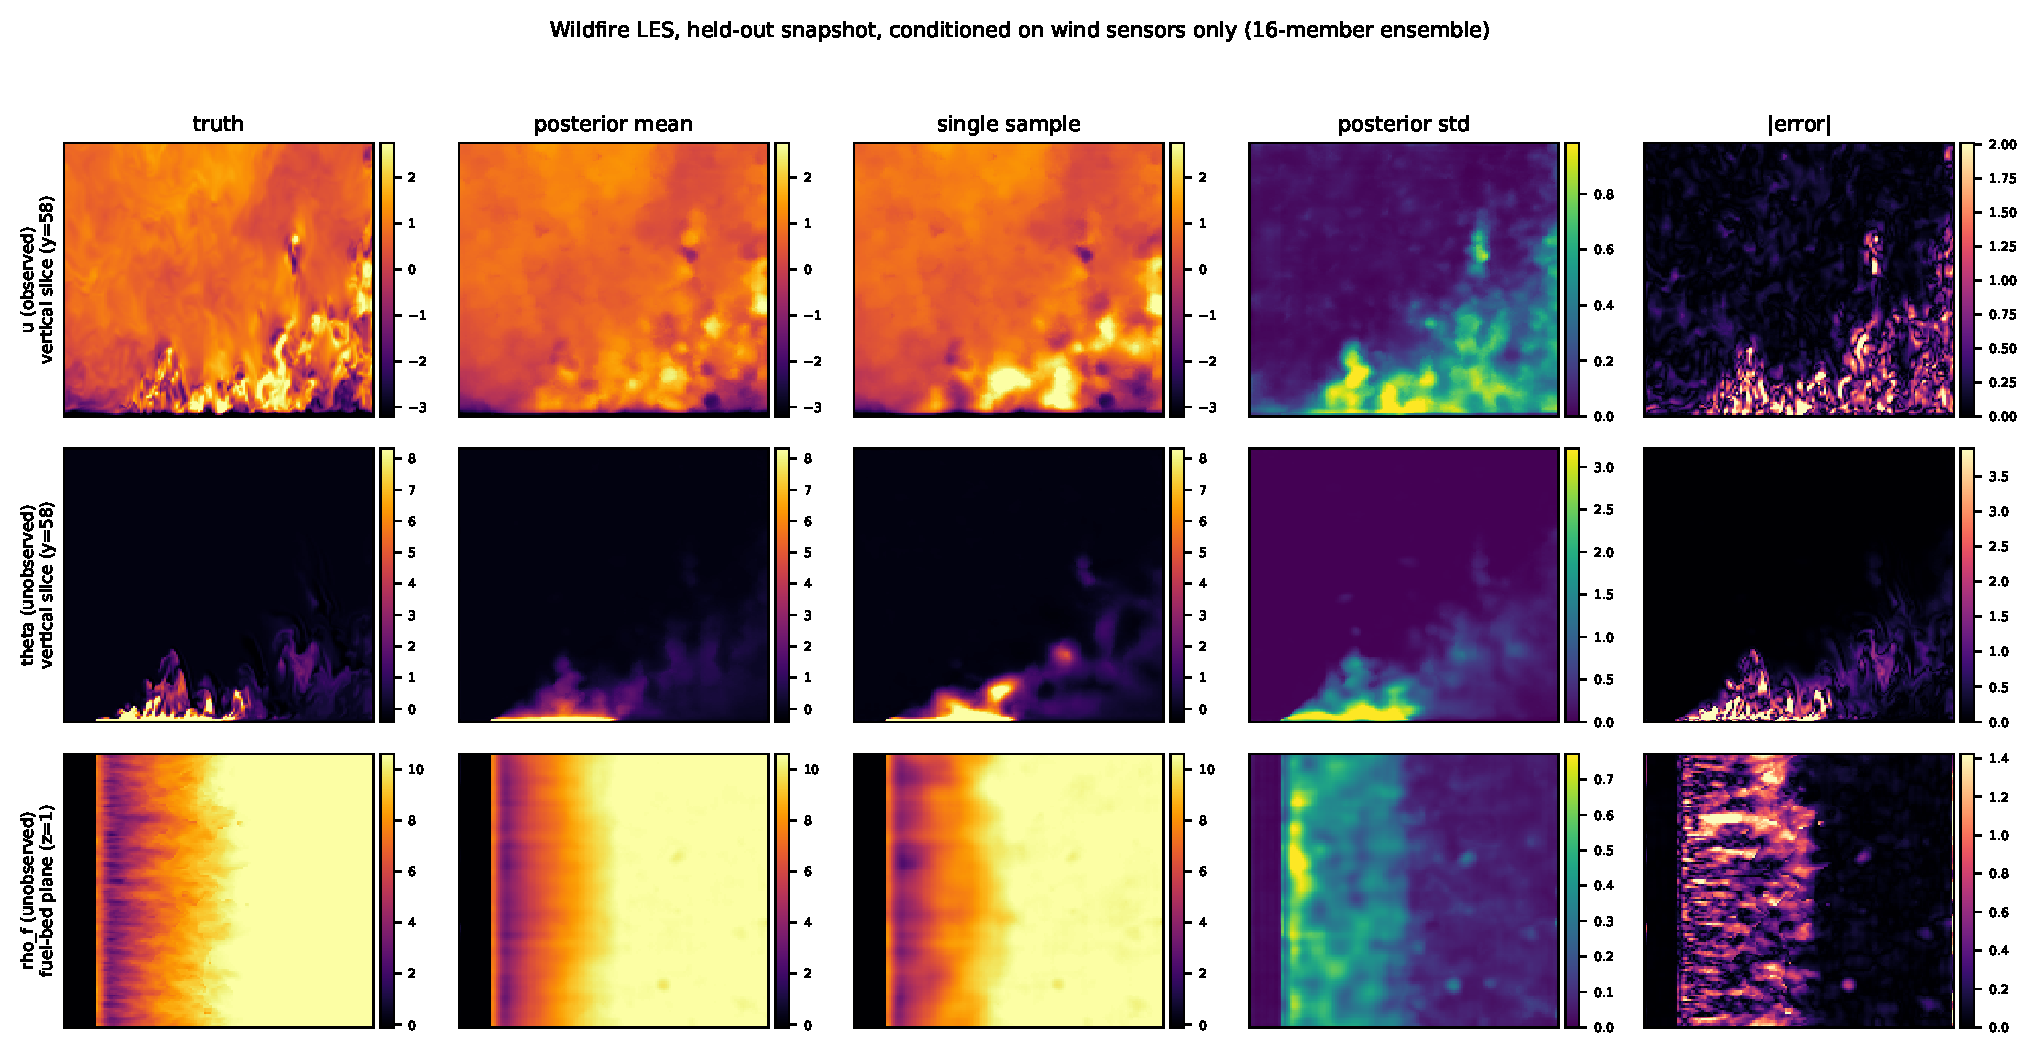
\includegraphics[width=\linewidth]{figures/qual_firebench.pdf}
\caption{\label{fig:qual-fb}Wildfire LES, held-out snapshot, conditioned on
wind sensors only (\dmfgen{}). Wind and potential temperature on a vertical
slice through the plume; fuel density on the fuel-bed plane. Potential
temperature and fuel density are never observed; from wind alone the model
localizes the burn scar, and the predictive standard deviation concentrates
exactly on the front.}
\end{figure}

% ---- cut from sec:wing (entire subsection incl. fig:qual-wing), 2026-09-08 ----
\subsection{Unstructured geometry with surface-only sensing}\label{sec:wing}

The wing is the capability filter: an unstructured mesh whose geometry varies
across cases, and observations confined to the body surface. Voxel diffusion,
patchified transformers, and latent-grid flow matching cannot be trained here
without resampling the adaptive mesh onto an axis-aligned grid --- a lossy
step that erases exactly the near-wall resolution the mesh exists to provide
--- so their rows are reported as \emph{not applicable without resampling}
rather than silently omitted; point-native methods (Senseiver, CoNFiLD-class
neural fields, SiT-point, gappy POD on the mesh, \dmfgen{}) compete fairly.
From 640 surface sensors (512 pressure taps, 128 shear gauges, Mach and
incidence as parameter tokens), \dmfgen{} recovers the volumetric
pressure-coefficient field on held-out geometries at 0.126 relative $L_2$ and
velocities at 0.53--0.69 (CRPS 0.18, spread--error 0.68, coverage 0.38;
$K{=}4$, NFE 4), with predictive standard deviation concentrating in the
boundary layer and wake --- the regions genuinely undetermined by surface
data (Fig.~\ref{fig:qual-wing}). \todo{wing baseline table (Senseiver,
SiT-point, MLP-RBF, gappy POD, IDW rows + n/a rows) --- the runs are
inventoried in the gap analysis and queue behind the 2D fleet.}

\begin{figure}[tbp]
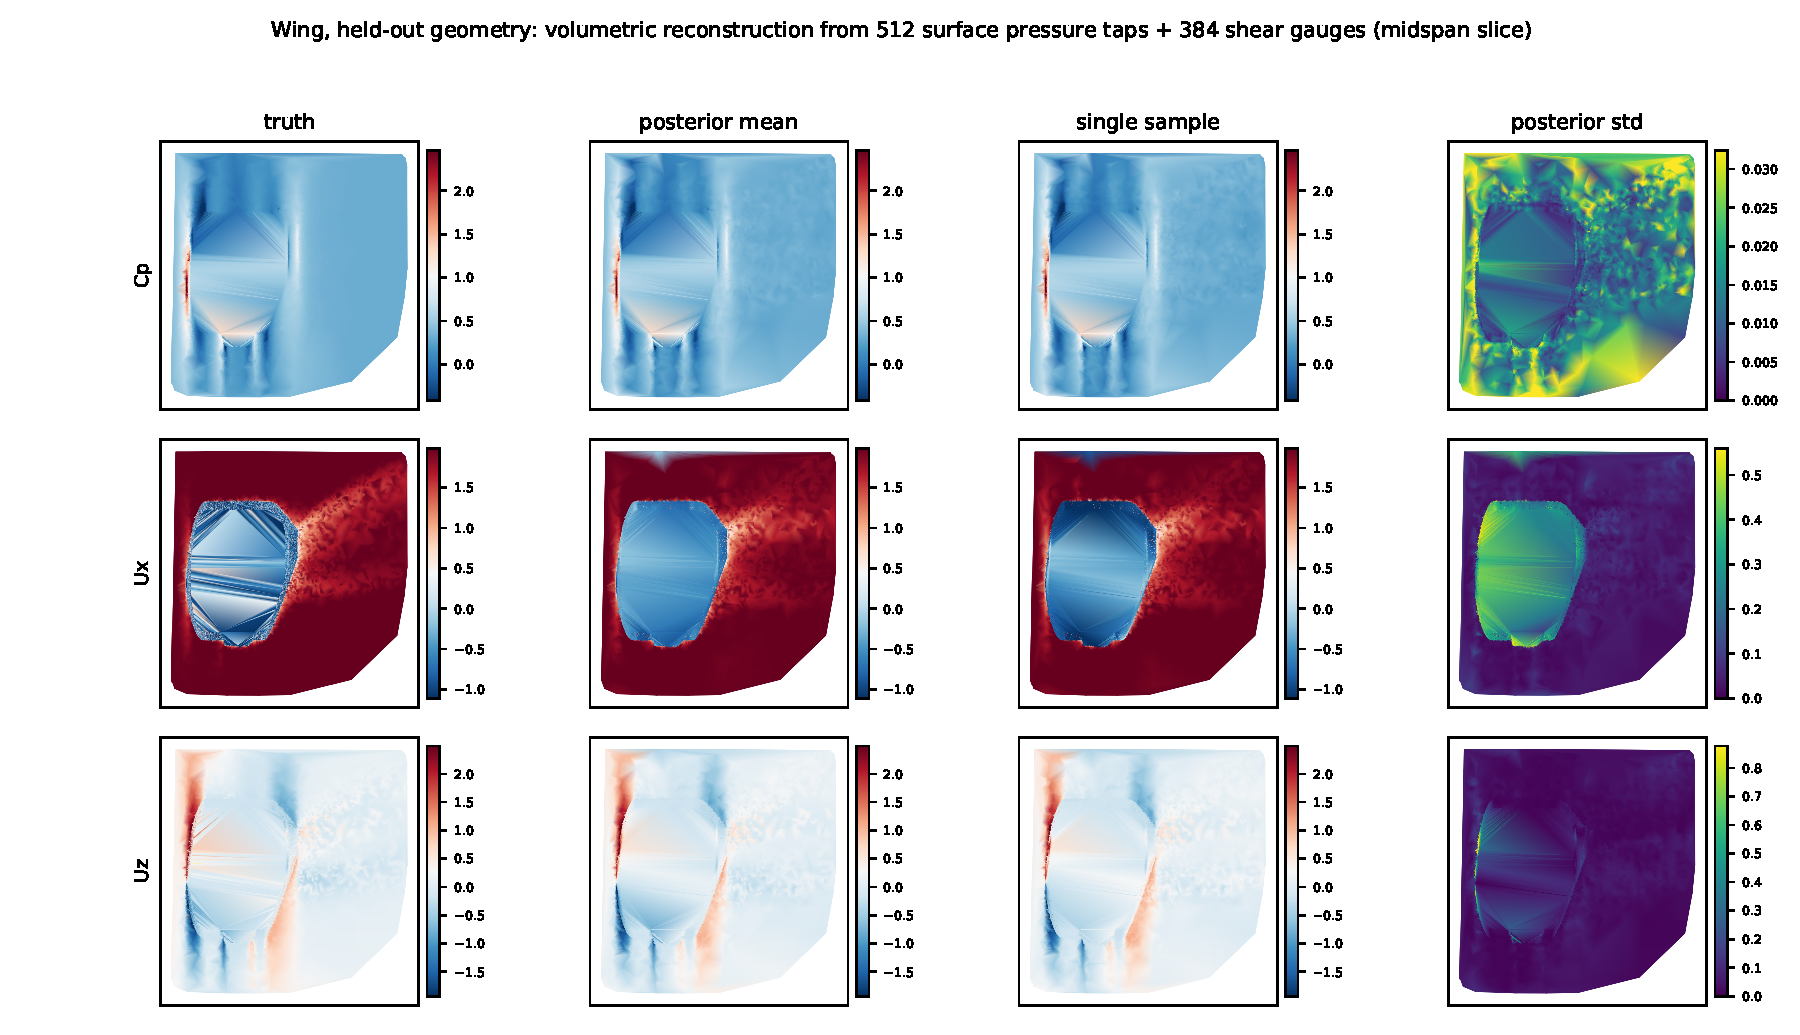
\includegraphics[width=\linewidth]{figures/qual_wing.pdf}
\caption{\label{fig:qual-wing}Wing, held-out geometry, midspan slice:
volumetric reconstruction from surface pressure taps and shear gauges alone
(\dmfgen{}). The predictive standard deviation is largest in the boundary
layer and wake, and spread and error decay together away from the skin
(pointwise correlation 0.77).}
\end{figure}

% ---- cut from fig:pareto caption (sec:cost), clause, 2026-09-08 ----
% Original clause "the operator matrix of Table~\ref{tab:ops}" was dropped from the caption.
the operator matrix of Table~\ref{tab:ops}) are where the grid-locked

% ---- cut from sec:kolmogorov, \todo clause, 2026-09-08 ----
% The clause "operator variants ported down from the FireBench matrix" was reworded to "operator variants (Sec.~\ref{sec:sensors})".
\todo{Senseiver/MLP-RBF/GeoFNO/S3GM rows (training/eval in queue); paired
CIs; spectra panel; operator variants ported down from the FireBench
matrix.}

% ---- cut from acknowledgments, \todo clause, 2026-09-08 ----
% FireBench and SHIFT-WING dataset providers removed from the acknowledgments \todo in main.tex; re-add in the follow-up.
\todo{funding/compute acknowledgments; DMF-Gen authors; JHTDB, FireBench,
SHIFT-WING dataset providers.}
